\begin{frame}
 \frametitle{Статистический сбор образцов: общие соображения}
 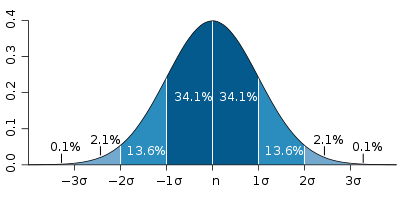
\includegraphics[width=0.7\textwidth]{../../slides/profile/Standard_deviation_diagram.png}
 \begin{itemize}
   \item Распределение Пуассона, в пределе больших $n$ переходящее в нормальное распределение
   \item Ширина распределения $\sim \sqrt{n}$
 \end{itemize}
\end{frame}

\begin{frame}
 \frametitle{Компоненты oprofile}
  \begin{itemize}
    \item Модуль ядра oprofile
    \item Системный демон \texttt{oprofiled}
    \item Программы управления \texttt{opcontrol,opannotate,}
  \end{itemize}
\end{frame}


\begin{frame}[fragile]
 \frametitle{Запуск oprofile: Проверка поддержки в ядре}
 \begin{itemize}
   \item \verb+ grep OPROFILE <configure>+
   \item Где найти \texttt{.configure}
     \begin{itemize}
      \item \texttt{.configure} В исходниках ядра
      \item \verb+/boot/configure-`uname -r`+
      \item \verb+/proc/config.gz+
     \end{itemize}
  \end{itemize}
\end{frame} 


\begin{frame}[fragile]
 \frametitle{Запуск oprofile: Работа}
 \begin{itemize}
  \item \verb+ opcontrol --vmlinux=/boot/vmlinux-3.2.xxx+ 
  \item \verb+ opcontrol --init+
  \item \verb+ opcontrol --start; ./my_program ; opcontrol --dump;  opcontrol --stop+
  \item \verb+ opannotate --source ./my_program +
 \end{itemize}
\end{frame}

\begin{frame}
 \frametitle{Упражнение}
 \begin{enumerate}
  \item Проверить, что в конфигурации ядра есть поддержка oprofile
  \item Скомпилировать программу с \texttt{-g}
  \item Запустить под oprofile
  \item Посмотреть статистику вызовов
  \item Запустить еще раз
  \item Посмотреть статистику еще раз, сравнить
 \end{enumerate}
\end{frame}
